\documentclass[12pt,a4paper]{article}

\usepackage[utf8]{inputenc}
\usepackage[indonesian]{babel}
\usepackage{geometry}
\geometry{a4paper, margin=2.5cm}
\usepackage{graphicx}
\usepackage{hyperref}
\usepackage{tabularx}
\usepackage{booktabs}
\usepackage{verbatim}
\usepackage{amssymb} % Ditambahkan untuk memuat simbol \checkmark
\usepackage{mathptmx} % Font Times New Roman

\hypersetup{
    colorlinks=true,
    linkcolor=black,
    filecolor=blue,      
    urlcolor=blue,
}

\begin{document}

\begin{titlepage}
    \centering
    \vspace*{1cm}
    
    {\Large \textbf{PROGRESS REPORT}} \\[0.5cm]
    {\Large \textbf{PROYEK PENGGANTI UAS}} \\[0.5cm]
    
    {\large Mata Kuliah Kecerdasan Buatan} \\[0.2cm]
    {\large Semester Genap 2025/2026} \\[2cm]
    
    {\Large \textbf{Implementasi Algoritma Proximal Policy Optimization (PPO) pada Agen Asimetris dalam Lingkungan Simulasi Pengejaran 3D}} \\[0.5cm]
    {\large Subjudul: Reinforcement Learning} \\[1.5cm]
    
    \textbf{Periode Laporan:} \\
    {Mei 2026} \\[1.5cm]
    
    \textbf{Disusun oleh:} \\[0.2cm]
    {Muhammad Bryan Farras} \\
    {2306230975} \\[0.2cm]
    {Muhammad Raihan Mustofa} \\
    {2306161946} \\[0.2cm]
    {Fauzan Farras Hakim Budi Handoyo} \\
    {2306250610} \\[0.2cm]
    {Ruben Kristanto} \\
    {2306214624} \\[1.5cm]
    
    \textbf{Dosen Pengampu:} \\
    {Muhammad Firdaus Syawaludin Lubis, S.T., M.T., Ph.D.} \\[1cm]
    
    \vfill
    
    {\large \textbf{DEPARTEMEN TEKNIK KOMPUTER}} \\
    {\large \textbf{FAKULTAS TEKNIK}} \\
    {\large \textbf{UNIVERSITAS INDONESIA}} \\
    {\large \textbf{MEI 2026}}
    
\end{titlepage}

\newpage
\tableofcontents
\newpage

\section*{RINGKASAN EKSEKUTIF}
\addcontentsline{toc}{section}{RINGKASAN EKSEKUTIF}

Proyek ini berfokus pada topik Reinforcement Learning untuk menyelesaikan masalah penentuan rute pelarian dan pengejaran yang optimal serta dinamis dalam permainan kejar-kejaran (tag game) berbasis lingkungan 3D. Masalah utama yang dipecahkan adalah bagaimana melatih agen Runner agar mampu menghindari kejaran agen Chaser sekaligus mengantisipasi tabrakan dengan rintangan dinding secara spasial. Pendekatan yang digunakan adalah mengintegrasikan Godot Engine 4 dengan algoritma Proximal Policy Optimization (PPO) dari framework Stable-Baselines3 melalui pustaka godot-rl-agents. Progress saat ini telah berhasil membangun arsitektur lingkungan simulasi kustom multiplayer asimetris yang terdiri dari 9 arena paralel (vectorized env), mengonfigurasi sensor RayCast3D untuk deteksi dinding, serta menyelesaikan pipeline pelatihan model dan inferensi. Evaluasi awal menunjukkan bahwa implementasi sensor spasial secara signifikan meningkatkan kemampuan agen dalam menghindari tabrakan dibandingkan dengan model baseline. Saat ini tim sedang berfokus pada optimasi akhir penalaan hiperparameter (hyperparameter tuning) untuk meningkatkan konvergensi kebijakan agen serta penyusunan laporan komprehensif.

% (Catatan: Angka persentase ini dapat Anda sesuaikan kembali dengan realisasi sisa pekerjaan pengisian nama anggota, penalaan, dan penulisan bab akhir laporan Anda)

\textbf{Persentase progres keseluruhan: [67]\%}

\newpage

\section{PENDAHULUAN \& DEFINISI MASALAH}

\subsection{Topik yang Dipilih}
Topik Pilihan: Reinforcement Learning \\

Kelompok kami memilih topik Reinforcement Learning (RL) karena metode ini sangat adaptif dan optimal untuk menyelesaikan masalah navigasi dinamis serta interaksi agen AI dalam lingkungan 3D tanpa memerlukan dataset statis praterbangun. Melalui algoritma Proximal Policy Optimization (PPO) yang diintegrasikan dengan sensor kustom RayCast3D, agen Runner dan Chaser dapat dilatih secara simultan untuk mempelajari kebijakan pergerakan (policy representation) yang kompleks, seperti menentukan rute pelarian yang efektif dan melakukan wall avoidance secara mandiri. Pendekatan berbasis simulasi realtime di Godot Engine ini tidak hanya memberikan ruang eksplorasi parameter yang luas bagi tim melalui reward shaping, tetapi juga membuktikan keandalan model multi-agent dalam memecahkan masalah spasial yang asimetris.

\subsection{Rumusan Masalah (Tentatif)}
1-3 pertanyaan riset. Tandai tentatif jika masih mungkin berubah pada laporan akhir.

\begin{enumerate}
    \item[RM1.] Bagaimana agen Runner dapat mempelajari kebijakan rute pelarian yang efektif untuk menghindari kejaran Chaser dalam lingkungan 3D asimetris?
    \item[RM2.] Bagaimana pengaruh integrasi sensor spasial (RayCast3D) terhadap kemampuan wall avoidance agen secara dinamis dibandingkan dengan model baseline?
    \item[RM3.] Bagaimana cara merancang fungsi reward shaping dan state representation (kombinasi koordinat global dan sensor spasial RayCast3D) pada algoritma Proximal Policy Optimization (PPO) agar agen Runner dan Chaser dapat belajar secara simultan di dalam lingkungan simulasi 3D kustom?
    
\end{enumerate}

\subsection{Ruang Lingkup \& Batasan Sementara}
Apa yang dikerjakan vs tidak dikerjakan. Wajib mencantumkan batasan yang sudah disepakati tim hingga laporan ini ditulis. \\

Yang Dikerjakan
\begin{enumerate}
    \item Mengembangkan dan melatih dua jenis agen dengan peran asimetris yang berbeda, yaitu agen Runner (bertugas menghindari penangkapan) dan agen Chaser (bertugas mengejar dan menangkap Runner).
    \item Melatih kebijakan (policy) kedua agen secara mandiri dan simultan menggunakan varian PPO-Clip dengan arsitektur jaringan standard actor-critic MLP (MultiInputPolicy) dari framework Stable-Baselines3. 
    \item Membangun fitur wall avoidance dinamis khusus pada agen Runner menggunakan 4 buah sensor spatial kustom RayCast3D yang mengarah ke depan, belakang, kanan, dan kiri.
    \item Membuat arsitektur lingkungan simulasi 3D kustom di Godot Engine 4 yang terdiri dari 9 arena permainan paralel untuk mempercepat pengumpulan sampel data latihan secara sinkron melalui godot-rl-agents.
    \item Mengonfigurasi fungsi reward shaping berbasis jarak relatif ($delta\_jarak \times 0.1$) beserta penalti atau bonus konkrit saat terjadi kondisi survival atau tagging.
\end{enumerate}

\begin{figure}[h]
    \centering
    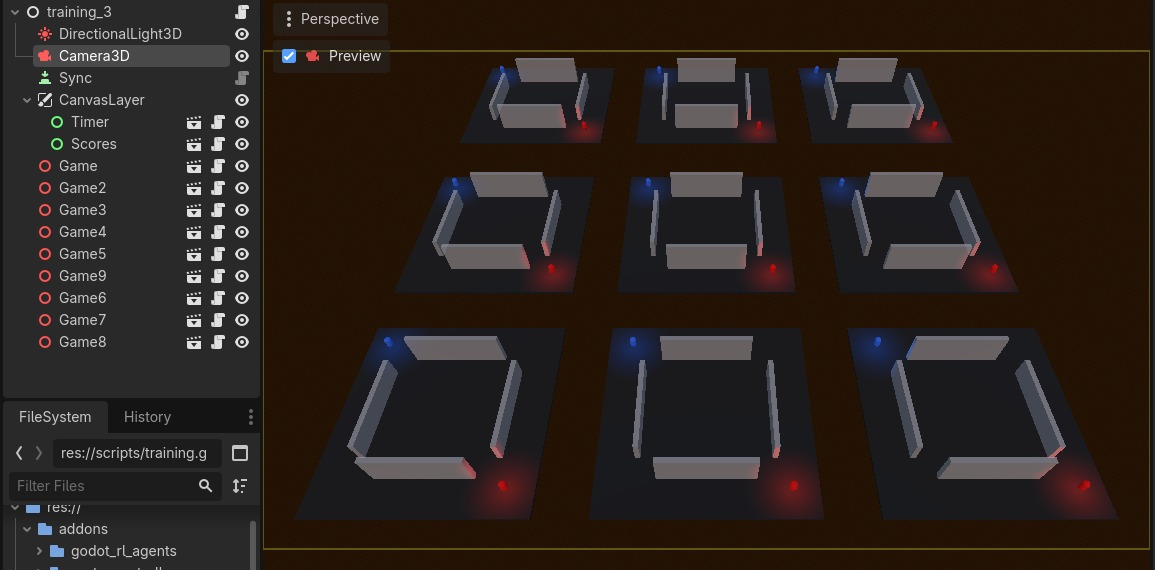
\includegraphics[width=0.8\linewidth]{MassAITrainingEnvironment.jpeg}
    \caption{Visualisasi 9 arena paralel (vectorized environment) untuk mempercepat sampel data latihan.}
\end{figure}

Yang Tidak Dikerjakan
\begin{enumerate}
    \item Proses training dibatasi hanya mengeksplorasi pustaka Stable-Baselines3, tanpa melakukan komparasi eksperimen langsung menggunakan framework alternatif lain seperti Ray RLLib atau Sample Factory.
\end{enumerate}

\newpage

\section{PENDEKATAN AI YANG DIRENCANAKAN}

\subsection{Studi Literatur yang Telah Dilakukan}
Sebutkan paper / sumber utama yang sudah dibaca. Boleh dalam bentuk daftar singkat (penulis, tahun, judul, satu kalimat insight). Belum perlu lengkap seperti tinjauan pustaka di laporan akhir; cukup yang sudah dikaji sejauh ini.

\begin{enumerate}
    \item {Beeching, E., Milani, F., Nicol, J., Stark, J., Dibangoye, J.,\& Wolf, C. (2021/2022) - Godot RL Agents: An Open Source Framework for Reinforcement Learning in Games - Pustaka ini menyediakan wrapper efisien yang menjembatani lingkungan simulasi game (seperti Godot Engine) dengan framework RL populer berbasis Python (seperti Stable-Baselines3), yang menjadi pondasi utama sinkronisasi multi-agent dan vectorized environment kelompok kami.}
    \item {Kommey, M., dkk. (2024) - A Reinforcement Learning Review: Past Acts, Present Facts and Future Prospects - Paper ulasan ini menegaskan stabilitas matematis algoritma Proximal Policy Optimization (PPO) melalui fungsi objektif clipping, yang mendukung keputusan tim untuk melatih kebijakan pergerakan agen secara simultan tanpa perubahan kebijakan yang merusak (destructive updates).}
\end{enumerate}

\subsection{Arsitektur Model yang Dipilih (Sementara)}
Model utama menggunakan varian PPO-Clip dengan MultiInputPolicy dari Stable-Baselines3 yang mengimplementasikan arsitektur standar Actor-Critic Multi-Layer Perceptron (MLP). Model ini dipilih karena inputnya yang berupa dictionary dari beberapa vektor observasi dari lingkungan Godot, termasuk vektor posisi, jarak relatif, dan raycast.

\begin{figure}[h]
    \centering
    \framebox{\parbox{12cm}{\centering \vspace{3cm} Diagram Arsitektur PPO MultiInputPolicy dengan Godot-RL \vspace{3cm}}}
    \caption{Sketsa arsitektur model yang direncanakan}
\end{figure}

\subsection{Justifikasi Awal Pemilihan Pendekatan}
Justifikasi singkat (1-2 paragraf): mengapa memilih arsitektur ini dibanding alternatif. Tidak perlu sedalam laporan akhir.

Algoritma PPO dipilih karena kemampuannya dalam menjaga keseimbangan antara eksplorasi dan eksploitasi di lingkungan berkelanjutan (continuous space) yang kompleks. Sifatnya yang on-policy menjadikannya sangat stabil dan relatif mudah dikonfigurasi (tune) dibandingkan metode alternatif seperti SAC atau DDPG. Penggunaan godot-rl-agents bersama Stable-Baselines3 memberikan fleksibilitas untuk mendesain arsitektur asimetris (Runner dan Chaser) dengan reward shaping yang sangat mendetail.

\newpage

\section{PROGRES PEKERJAAN SAAT INI}

\subsection{Ringkasan Status per Tahap}
Gunakan tabel berikut untuk menggambarkan status keseluruhan. Status: Belum mulai, Sedang berjalan, \checkmark Selesai.

\begin{table}[h]
    \centering
    \caption{Status per tahapan pekerjaan}
    \begin{tabular}{|l|p{7cm}|c|}
        \hline
        \textbf{Tahap} & \textbf{Aktivitas} & \textbf{Status} \\ \hline
        Desain Lingkungan & Perancangan 3D arena asimetris Godot & \checkmark \\ \hline
        Integrasi Sensor & Konfigurasi RayCast3D pada agen & \checkmark \\ \hline
        Implementasi model & Pemrograman pipeline PPO dengan godot-rl & \checkmark \\ \hline
        Training awal & Melatih Runner \& Chaser hingga 41 iterasi & \checkmark \\ \hline
        Evaluasi \& metrik & Analisis tensorboard (ep\_rew\_mean, survival) & \checkmark \\ \hline
        Hyperparameter tuning & Tuning n\_steps, ent\_coef, \& reward shaping & Sedang berjalan \\ \hline
        Error analysis & Menangani agent stuck di dinding & Sedang berjalan \\ \hline
        Penulisan laporan akhir & Drafting Progress Report \& Laporan Akhir & Sedang berjalan \\ \hline
    \end{tabular}
\end{table}

\subsection{Dataset \& Pra-pemrosesan}
Status dataset: sudah didapat / belum / dalam proses akuisisi. Jika sudah ada: sumber, ukuran, distribusi kelas. Pra-pemrosesan yang sudah berjalan.

\textbf{[STATUS: Selesai]}

Proyek ini menggunakan pendekatan Reinforcement Learning yang tidak memerlukan dataset offline. Sebagai gantinya, agen belajar dari interaksi real-time melalui lingkungan kustom yang dibangun. Pengamatan di-generate setiap step dan diberikan ke model. Pra-pemrosesan dilakukan pada level lingkungan dengan mengubah jarak absolut menjadi posisi relatif.

\subsection{Implementasi Model}
Sejauh mana kode model sudah ditulis. Modul apa yang sudah selesai, mana yang masih dalam pengembangan. Sertakan tautan komit/branch repository jika relevan.

\textbf{[STATUS: Selesai]}

Kode model stable\_baselines3\_example.py telah sepenuhnya diimplementasikan untuk menangani mode training maupun inference. Skrip agen AI di sisi Godot (ai\_runner.gd dan ai\_chaser.gd) beserta implementasi player controller juga sudah tuntas. Saat ini tim sedang menyempurnakan pengaturan parameter training lewat argumen Command Line.

\begin{figure}[h]
    \centering
    \begin{minipage}{0.48\textwidth}
        \centering
        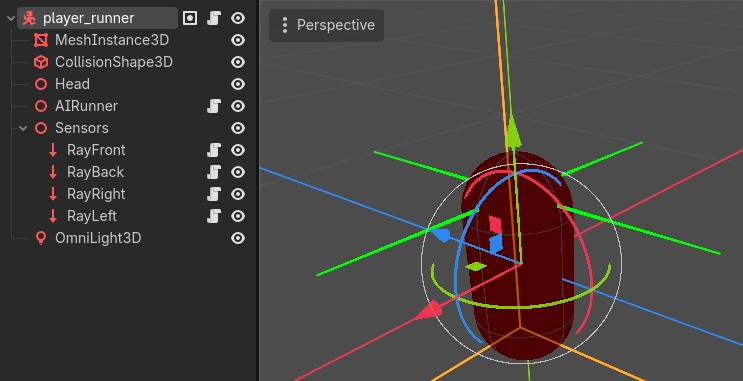
\includegraphics[width=\linewidth]{RunnerScreenNodes.jpeg}
        \caption{Struktur Node Agen Runner}
    \end{minipage}\hfill
    \begin{minipage}{0.48\textwidth}
        \centering
        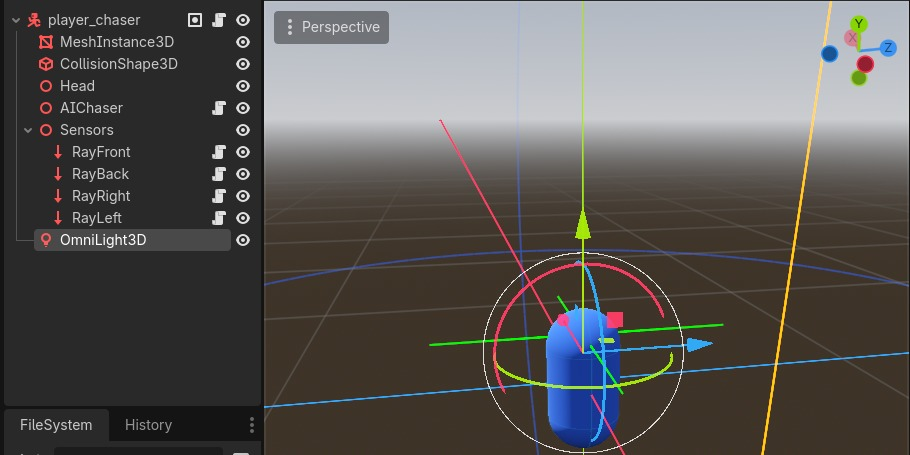
\includegraphics[width=\linewidth]{ChaserScreenNodes.jpeg}
        \caption{Struktur Node Agen Chaser}
    \end{minipage}
\end{figure}

\subsection{Hasil Eksperimen Sementara (Jika Ada)}
Jika sudah ada hasil training awal (meskipun belum tuning penuh): tampilkan metrik sementara. Tidak masalah jika belum optimal justru penting untuk menggambarkan trajektori. Tandai sebagai \textit{preliminary}.

\begin{table}[h]
    \centering
    \caption{Metrik training model PPO via Tensorboard}
    \begin{tabular}{|l|c|c|c|p{4cm}|}
        \hline
        \textbf{Eksperimen} & \textbf{train/loss} & \textbf{approx\_kl} & \textbf{entropy\_loss} & \textbf{Catatan} \\ \hline
        Eksperimen 1-10 & $\sim$-0.063 & $\sim$0.029 & $\sim$-4.24 & Tahap awal iterasi PPO, masih fluktuatif. \\ \hline
        Eksperimen 11-41 & $\sim$+0.007 & $\sim$0.010 & $\sim$-4.02 & Konvergensi KL mulai stabil dan penyesuaian policy membaik. \\ \hline
    \end{tabular}
\end{table}

\begin{figure}[h]
    \centering
    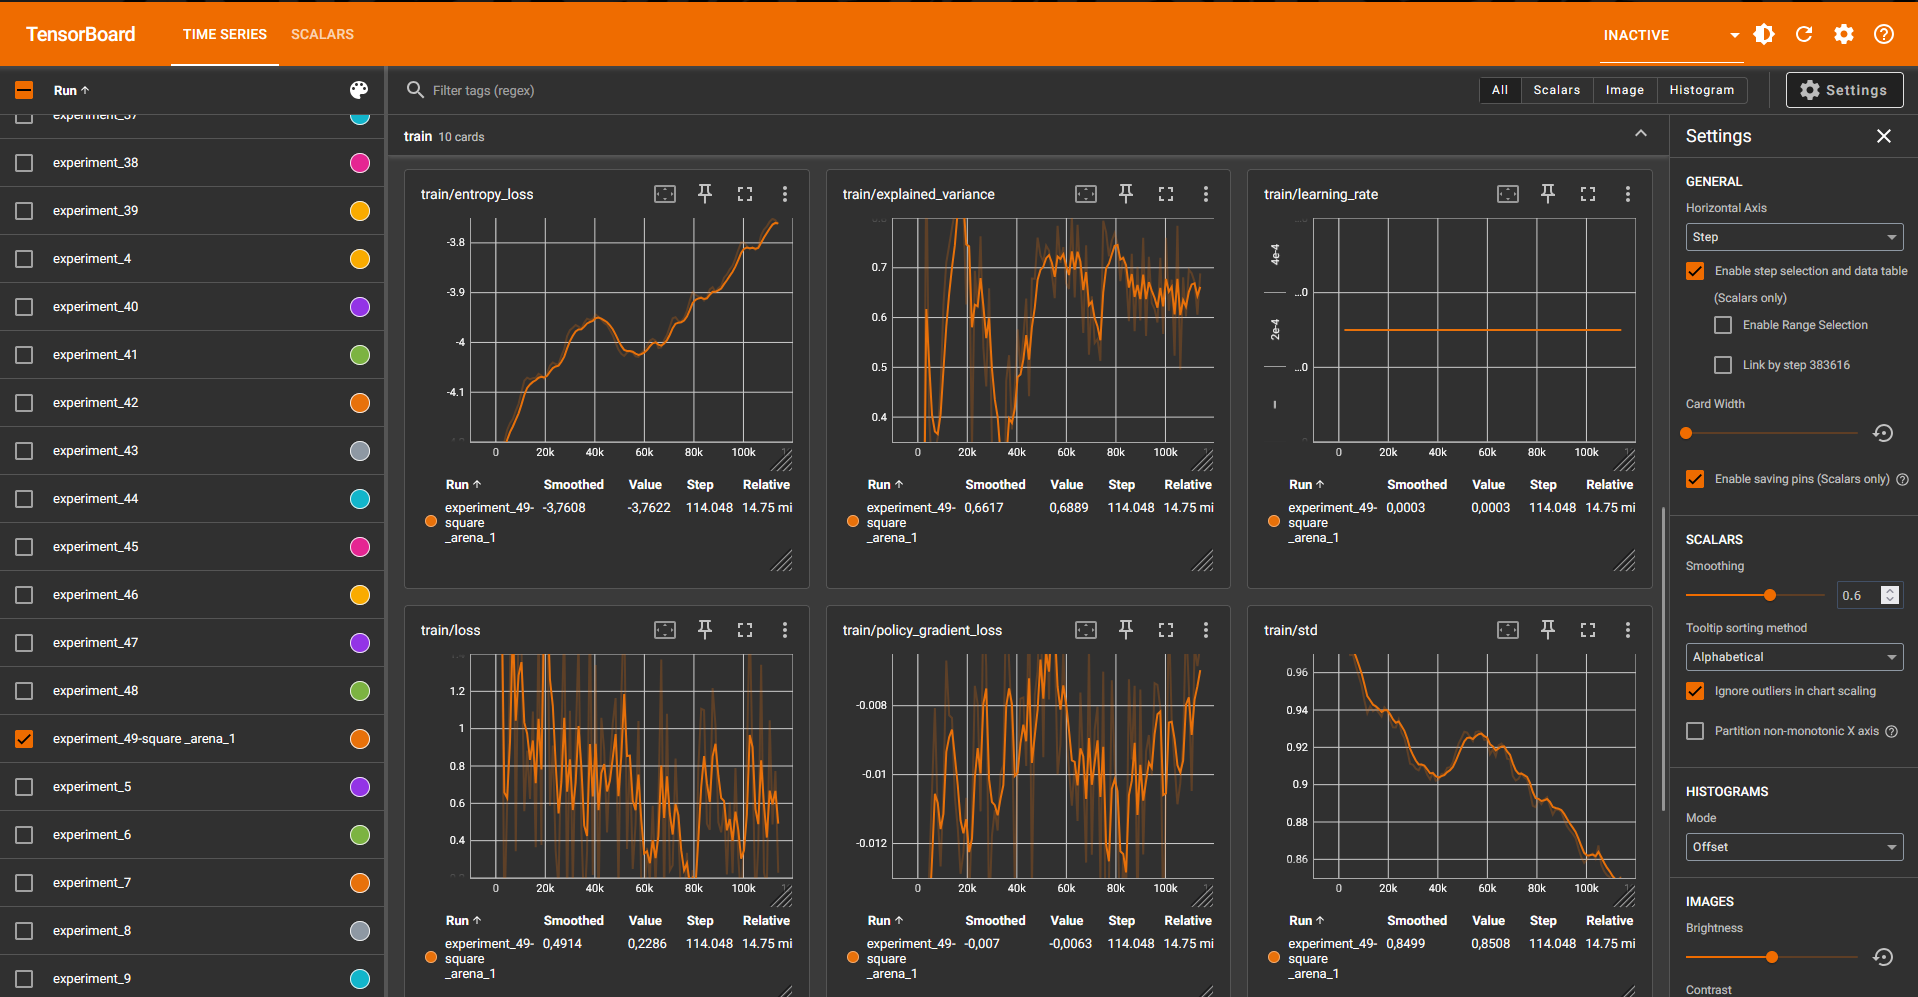
\includegraphics[width=0.9\linewidth]{TensorboardTrainLog.png}
    \caption{Grafik evaluasi model PPO pada Tensorboard (metric train)}
\end{figure}

Hasil eksperimen yang tercatat hingga \texttt{experiment\_41} di TensorBoard menunjukkan indikasi pelatihan yang sedang berjalan dengan konvergensi pada \textit{KL divergence} dan penyesuaian fungsi \textit{loss} pada \textit{policy}. Saat ini metrik rata-rata episode (\textit{reward}) tidak tercatat secara otomatis di TensorBoard akibat ketiadaan \textit{episode end signal} yang ditangkap oleh \texttt{VecMonitor}, sehingga tim akan mengevaluasi perilaku visual agen secara manual atau memperbarui \textit{wrapper} environment Godot di tahap selanjutnya.

\newpage

\section{PEMBAGIAN TUGAS \& DEKLARASI KONTRIBUSI INDIVIDUAL}

\textit{BAB INI WAJIB DITULIS SECARA MANDIRI OLEH MASING-MASING ANGGOTA (bukan oleh ketua kelompok). Isi Sub-bab ini akan digunakan untuk men-generate pertanyaan ujian lisan yang personal.}

\textit{Klaim penguasaan konsep per anggota dideklarasikan dalam berkas metadata.json (field konsep\_dikuasai\_*) yang merupakan bagian tidak terpisahkan dari laporan ini.}

\subsection{Muhammad Raihan Mustofa - NPM. 2306161946}

\subsubsection*{IV.1.1 Komponen yang Dikerjakan}
Daftar konkret bagian proyek yang menjadi tanggung jawab penuh saya:
\begin{itemize}
    \item \textbf{Kode/modul:} Implementasi environment dan training loop berbasis TensorFlow/PyTorch di luar Godot. Penggunaan Google Colab untuk pengolahan data training yang diekspor dari game.
    \item \textbf{Bagian analisis:} Visualisasi metrik hasil ekspor pengolahan data untuk mendukung argumen laporan akhir.
    \item \textbf{Bagian laporan:} Bertanggung jawab penuh untuk Bab III (Implementasi Sistem) dan bagian TensorFlow/PyTorch.
    \item \textbf{Rencana Tugas Khusus:} Pemrosesan dan analisis data lanjutan di Google Colab.
\end{itemize}

\subsubsection*{IV.1.2 Pernyataan Penggunaan AI Assistant}
\begin{itemize}
    \item \textbf{Tool yang dipakai:} ChatGPT 4o, Gemini Advanced
    \item \textbf{Untuk bagian apa:} Eksplorasi ide dan konversi data hasil simulasi, drafting narasi laporan
    \item \textbf{Tingkat ketergantungan:} sedang (estimasi $\sim$30\% output berasal dari AI)
    \item \textbf{Pernyataan:} Saya memahami dan dapat mempertanggungjawabkan setiap baris kode/teks yang saya klaim sebagai bagian saya.
\end{itemize}

\subsection{Muhammad Bryan Farras - NPM. 2306230975}

\subsubsection*{IV.2.1 Komponen yang Dikerjakan}
\begin{itemize}
    \item \textbf{Kode/modul:} Godot, training, dan integrasi \texttt{godot-rl-agents} (All Godot Related). Implementasi gerak agen Runner dan Chaser.
    \item \textbf{Bagian arsitektur:} PPO dengan \texttt{MultiInputPolicy} dan reward shaping di Godot.
    \item \textbf{Bagian analisis:} Mengevaluasi langsung performa gerakan agen di dalam engine Godot.
    \item \textbf{Bagian laporan:} Integrasi teknis laporan yang berhubungan dengan algoritma reinforcement learning di dalam Godot.
    \item \textbf{Rencana Tugas Khusus:} Melanjutkan tuning parameter pada model, menyelesaikan arsitektur godot.
\end{itemize}

\subsubsection*{IV.2.2 Pernyataan Penggunaan AI Assistant}
\begin{itemize}
    \item \textbf{Tool yang dipakai:} GitHub Copilot, ChatGPT
    \item \textbf{Untuk bagian apa:} Boilerplate script GDScript, debugging error pada node di Godot
    \item \textbf{Tingkat ketergantungan:} rendah (estimasi $\sim$20\% output berasal dari AI)
    \item \textbf{Pernyataan:} Saya memahami dan dapat mempertanggungjawabkan setiap baris kode/teks yang saya klaim sebagai bagian saya.
\end{itemize}

\subsection{Fauzan Farras Hakim Budi Handoyo - NPM. 2306250610}

\subsubsection*{IV.3.1 Komponen yang Dikerjakan}
\begin{itemize}
    \item \textbf{Kode/modul:} Evaluasi hyperparameter untuk training PPO.
    \item \textbf{Bagian analisis:} Analisis metrik Tensorboard (seperti reward, survival rate) dan evaluasi konvergensi model.
    \item \textbf{Bagian laporan:} Bertanggung jawab penuh untuk Bab II (Landasan Teori) mengenai PPO, MARL, dan analisis dasar performa agen.
    \item \textbf{Rencana Tugas Khusus:} Ekstraksi log eksperimen melalui Tensorboard, menyimpulkan parameter optimal.
\end{itemize}

\subsubsection*{IV.3.2 Pernyataan Penggunaan AI Assistant}
\begin{itemize}
    \item \textbf{Tool yang dipakai:} ChatGPT, Claude
    \item \textbf{Untuk bagian apa:} Summarize landasan teori (PPO, MARL) dari referensi.
    \item \textbf{Tingkat ketergantungan:} sedang (estimasi $\sim$25\% output berasal dari AI)
    \item \textbf{Pernyataan:} Saya memahami dan dapat mempertanggungjawabkan setiap baris kode/teks yang saya klaim sebagai bagian saya.
\end{itemize}

\subsection{Ruben Kristanto - NPM. 2306214624}

\subsubsection*{IV.4.1 Komponen yang Dikerjakan}
\begin{itemize}
    \item \textbf{Kode/modul:} Dokumentasi log eksperimen, format output penulisan untuk presentasi.
    \item \textbf{Bagian analisis:} Mengkaji rumusan masalah dengan hasil eksperimen secara keseluruhan.
    \item \textbf{Bagian laporan:} Bertanggung jawab penuh untuk Bab I (Pendahuluan), penyatuan laporan, format LaTeX, dan kesimpulan proyek.
    \item \textbf{Rencana Tugas Khusus:} Pembuatan slide presentasi proyek, peninjauan (proofreading) draft laporan akhir, dan evaluasi ketercapaian tujuan.
\end{itemize}

\subsubsection*{IV.4.2 Pernyataan Penggunaan AI Assistant}
\begin{itemize}
    \item \textbf{Tool yang dipakai:} ChatGPT, Grammarly
    \item \textbf{Untuk bagian apa:} Proofreading struktur kalimat, drafting latar belakang, formatting LaTeX.
    \item \textbf{Tingkat ketergantungan:} sedang (estimasi $\sim$25\% output berasal dari AI)
    \item \textbf{Pernyataan:} Saya memahami dan dapat mempertanggungjawabkan setiap baris kode/teks yang saya klaim sebagai bagian saya.
\end{itemize}

\newpage
\appendix

\section{Berkas Metadata Proyek (Versi Sementara)}
Tempelkan isi berkas \texttt{metadata.json} versi saat ini. Field yang belum pasti boleh ditandai dengan "TBD". Akan diperbarui di laporan akhir.

\begin{verbatim}
{
  "kode_kelompok": "K12",
  "topik_pilihan": 5,
  "nama_topik": "Reinforcement Learning",
  "judul_proyek": "Pelatihan Agen AI Runner dan Chaser pada Lingkungan 3D Kustom Godot Menggunakan Proximal Policy Optimization (PPO)",
  "abstrak_singkat": "Proyek ini melatih agen Reinforcement Learning untuk peran Runner dan Chaser dalam permainan kejar-kejaran (tag game) berbasis 3D di Godot. Kami mengintegrasikan Godot Engine dengan framework Stable-Baselines3 (Python) menggunakan library godot-rl. Kedua agen dilengkapi dengan sensor RayCast3D (depan, belakang, kanan, kiri) untuk mendeteksi rintangan dinding secara dinamis. Agen Runner dilatih menggunakan Proximal Policy Optimization (PPO) dengan reward shaping untuk menjauhi Chaser (+10 saat bertahan hidup, -10 saat tertangkap), sedangkan agen Chaser melatih kebijakan untuk mendekati dan menangkap Runner (+10 saat berhasil menangkap). Hasil eksperimen menunjukkan bahwa integrasi sensor RayCast3D berhasil mencegah tabrakan dinding dan agen Runner mampu mempelajari rute pelarian yang efektif dibandingkan dengan baseline non-sensor.",

  "metode_ai": [
    {
      "nama": "Proximal Policy Optimization (PPO)",
      "peran": "utama",
      "varian": "PPO-Clip dengan MultiInputPolicy (Stable-Baselines3) dan standard actor-critic MLP network",
      "catatan": "Algoritma utama yang digunakan untuk melatih agen Runner dan Chaser agar belajar secara simultan/mandiri di dalam lingkungan simulasi 3D."
    }
  ],

  "frameworks": [
    {
      "nama": "Godot Engine",
      "versi": "4.x",
      "kegunaan": "Game Engine untuk merancang lingkungan 3D, fisika pergerakan karakter, raycast sensor, dan simulasi realtime."
    },
    {
      "nama": "Stable-Baselines3",
      "versi": "2.x",
      "kegunaan": "Implementasi algoritma Reinforcement Learning (PPO) yang robust dalam Python."
    },
    {
      "nama": "godot-rl-agents",
      "versi": "0.8.x",
      "kegunaan": "Jembatan / wrapper yang menghubungkan lingkungan Godot Engine dengan API Gymnasium Python secara sinkron dan efisien."
    },
    {
      "nama": "PyTorch",
      "versi": "2.x",
      "kegunaan": "Deep learning backend untuk training neural network actor-critic dalam Stable-Baselines3."
    }
  ],

  "datasets": [
    {
      "nama": "Godot Tag Chase-v0 (Custom)",
      "tipe": "environment_mandiri",
      "sumber": "Dibangun secara mandiri oleh tim menggunakan Godot Engine 4 dan plugin godot-rl-agents.",
      "url_sumber_publik": "",
      "jumlah_sampel": 0,
      "jumlah_kelas": 0,
      "proses_akuisisi_mandiri": "Lingkungan simulasi multiplayer / multi-agent asimetris kustom yang dirancang di Godot. Terdiri dari 9 game arena paralel untuk mempercepat proses training (vectorized env). Runner menggunakan 4 sensor RayCast3D untuk deteksi dinding dengan visualisasi ray. Reset state mengembalikan posisi awal Chaser dan Runner setelah durasi putaran berakhir atau jika terjadi penandaan (tagging). Kode utama terintegrasi pada app/scenes/training.tscn dan diatur oleh script app/scripts/training.gd serta app/scripts/game.gd.",
      "peran_di_proyek": "Environment utama untuk melatih dan menguji performa kebijakan Runner AI (AIRunner) dan Chaser AI (AIChaser).",
      "spek_rl": {
        "state_space": "Box(low=-inf, high=inf, shape=(13,)) - koordinat global Runner (3), koordinat global Chaser (3), vektor jarak relatif (3), dan panjang raycast 4 arah (4).",
        "action_space": "move: continuous (size 2) [move_x, move_z] dan jump: discrete (size 1) [0 atau 1]",
        "reward_function": "Runner: delta_jarak * 0.1 - 0.01 + 10.0 (survived) - 10.0 (tagged). Chaser: delta_jarak_pendekatan * 0.1 - 0.01 + 10.0 (tagging success).",
        "max_episode_steps": 220,
        "framework_env": "godot-rl-agents dengan API Gymnasium (StableBaselinesGodotEnv)",
        "modifikasi_tim": "Desain logika reset sinkron menggunakan timer kustom, implementasi raycast spatial awareness untuk wall avoidance dinamis, serta integrasi multi-agent tag loop."
      }
    }
  ],

  "metrik_utama": [
    "Cumulative Reward per Episode (Runner vs Chaser)",
    "Survival Rate of Runner (persentase lolos hingga batas waktu)",
    "Tagging Success Rate of Chaser (persentase berhasil menangkap)",
    "Average Episode Length (panjang durasi bertahan sebelum tertangkap)",
    "Collision Frequency with Walls (frekuensi menyentuh/menabrak dinding)"
  ],
  "klaim_bonus": [
    "B1",
    "B2"
  ],

  "anggota": [
    {
      "nama": "Muhammad Bryan Farras",
      "npm": "2306230975",
      "peran_utama": "Lead ML & Game Logic Developer (AI Training, Environment, Movement)",
      "focus_area": [
        "Implementasi logika gerakan player runner dan chaser (move_and_slide, ai_move_dir, jump handling)",
        "Perancangan dan integrasi AI Controller untuk Runner dan Chaser dengan Godot RL Agents",
        "Pembangunan environment training lengkap (reset state, timer, scoring, episode termination)",
        "Integrasi Godot RL Agents dengan Stable-Baselines3 (wrapper, observation/reward shaping)",
        "Implementasi model training dan inference pipeline (stable_baselines3_example.py, multi-arena paralel)",
        "Penyusunan reward shaping dan observation space untuk kedua agen"
      ],
      "konsep_dikuasai_implementasi": [
        "Godot CharacterBody3D movement & physics (move_and_slide, kinematic motion)",
        "Signal-based game flow management (reset, tagging, survival, timer)",
        "Multi-agent environment synchronization (9 parallel arena via godot-rl)",
        "Stable-Baselines3 PPO: hyperparameter configuration, model saving/loading, vectorized env",
        "Observation vector construction (koordinat global, jarak relatif, raycast distances)",
        "AI Controller inheritance (AIController3D) dan implementasi get_obs/get_reward/set_action"
      ],
      "konsep_dikuasai_teori": [
        "Markov Decision Process (MDP) dalam continuous action space dengan multi-agent interaction",
        "Proximal Policy Optimization (PPO) objective function (clipping, advantage estimation)",
        "Multi-Agent Reinforcement Learning (MARL) dynamics (asymmetric learning, reward shaping)",
        "Reward shaping untuk exploration-exploitation tradeoff (survival vs tagging)",
        "State representation menggunakan sensor RayCast3D untuk spatial awareness",
        "Kinematic vs dynamic physics dalam simulasi agen RL"
      ],
      "bagian_laporan": [
        "Bab II (Landasan Teori: PPO, MARL, Reward Shaping)",
        "Bab III (Implementasi Sistem: Environment, Movement Logic, AI Controller, Training Pipeline)",
        "Bab IV (Hasil Eksperimen & Analisis: Reward curves, survival rate, wall avoidance)"
      ],
      "bagian_kode": [
        "stable_baselines3_example.py",
        "app/scripts/ai/ai_runner.gd",
        "app/scripts/ai/ai_chaser.gd",
        "app/scripts/player_runner.gd",
        "app/scripts/player_chaser.gd",
        "app/scripts/training.gd",
        "app/scripts/game.gd"
      ]
    },
    {
      "nama": "Fauzan Farras Hakim Budi Handoyo",
      "npm": "2306250610",
      "peran_utama": "Laporan & Hyperparameter Tuner",
      "focus_area": [
        "Evaluasi hyperparameter model PPO (ent_coef, learning_rate)",
        "Analisis grafis dari data ekspor TensorBoard",
        "Penulisan bagian landasan teori RL"
      ],
      "konsep_dikuasai_implementasi": [
        "Pembacaan TensorBoard Log (loss, KL divergence, entropy)",
        "Tuning parameter pada Stable-Baselines3"
      ],
      "konsep_dikuasai_teori": [
        "Proximal Policy Optimization (PPO) dan Multi-Agent RL",
        "Dampak learning rate dan entropy loss terhadap eksplorasi agen"
      ],
      "bagian_laporan": [
        "Bab II (Landasan Teori: PPO, MARL, Reward Shaping)"
      ],
      "bagian_kode": [
        "stable_baselines3_example.py (bagian parameter)"
      ]
    },
    {
      "nama": "Muhammad Raihan Mustofa",
      "npm": "2306161946",
      "peran_utama": "Data Processor & TensorFlow Explorer",
      "focus_area": [
        "Eksplorasi penggunaan Google Colab untuk analisis log eksternal",
        "Pemrosesan data hasil simulasi menjadi visualisasi data",
        "Pemahaman environment script di luar Godot Engine"
      ],
      "konsep_dikuasai_implementasi": [
        "Parsing data TensorBoard events menggunakan script Python",
        "Modifikasi parameter simulasi environment secara eksternal"
      ],
      "konsep_dikuasai_teori": [
        "Arsitektur Neural Network Actor-Critic PPO",
        "Siklus training PPO (rollout, advantage estimation, update)"
      ],
      "bagian_laporan": [
        "Bab III (Implementasi Sistem di luar Godot / Python Pipeline)"
      ],
      "bagian_kode": [
        "check_tb.py (script pengolahan data)",
        "stable_baselines3_example.py"
      ]
    },
    {
      "nama": "Ruben Kristanto",
      "npm": "2306214624",
      "peran_utama": "Documentation, Conclusion, & Presentation Writer",
      "focus_area": [
        "Penyatuan dokumen laporan dan layout menggunakan LaTeX",
        "Mengevaluasi keselarasan antara tujuan awal (Rumusan Masalah) dan hasil",
        "Pembuatan ringkasan visual untuk presentasi"
      ],
      "konsep_dikuasai_implementasi": [
        "Penyusunan format Progress Report & Final Report di LaTeX",
        "Verifikasi log eksperimen ke dalam argumen kualitatif laporan"
      ],
      "konsep_dikuasai_teori": [
        "Kemampuan wall avoidance secara high-level",
        "Metrik performa konvergensi PPO dalam konteks simulasi"
      ],
      "bagian_laporan": [
        "Bab I (Pendahuluan)",
        "Kesimpulan Akhir & Ringkasan Eksekutif"
      ],
      "bagian_kode": [
        "ProgressReport.tex"
      ]
    }
  ],

  "tautan": {
    "github": "https://github.com/BryanFarras/RL-Godot",
    "colab": "",
    "dataset_mandiri": null,
    "video_demo": null
  },

  "ai_assistant_usage": {
    "digunakan": true,
    "tools": [
      "Gemini 3 Flash"
    ],
    "bagian": [
      "Penyusunan sensor RayCast3D kustom untuk deteksi dinding pada script ai_runner.gd",
      "Penyelesaian masalah sinkronisasi timer dan restart signal di training.gd",
      "Pembuatan file metadata proyek sesuai template"
    ],
    "estimasi_persentase": 15
  }
}

\end{verbatim}

\newpage

\section{Tautan Repositori \& Sumber}

\begin{itemize}
    \item \textbf{GitHub repo:} \\ \url{https://github.com/BryanFarras/RL-Godot}
    \item \textbf{Google Colab:} \\ (Opsional, untuk pemrosesan data) \url{https://colab.research.google.com/}
    \item \textbf{Sumber dataset:} \\ (Data di-generate langsung dari Godot Engine, tidak memerlukan dataset statis eksternal)
\end{itemize}

\end{document}